% !Mode:: "TeX:UTF-8"

\documentclass[proposal]{zjutreport}
\usepackage{url}
\graphicspath{{figures/}}  % 定义所有的eps文件在 figures 子目录下
\begin{document}           % 开始全文

%论文题目:{中文}
\zjuttitle{基于内存数据库的大数据应用系统的设计与实现}
%作者:{中文姓名}{学号}
\zjutauthor{陈佳鹏}{200926630503}
%指导教师:{导师中文名}
\zjutmentor{陈~~~~波}
%个人信息:{毕业年份}{专业名称}
\zjutinfo{2013}{软件工程}
%学院信息:{学院中文}
\zjutcollege{计算机科学与技术学院}
%日期:{提交日期}
\zjutdate{2013年03月}

\input{preface/cover}      % 封面

\frontmatter

\pagenumbering{Roman}
\begingroup % 在组内的chapter不换行
\let\clearpage\relax % chapter之后不换页

%%%%%%%%%% 标题 %%%%%%%%%%
\titleformat{\chapter}[block]{\sihao\heiti\filcenter\bfseries}{\CJKnumber{\thechapter}}{1ex}{}{} % 标题居中,黑体三号
\chapter*{基于内存数据库的大数据应用系统的设计与实现}
\titleformat{\chapter}[block]{\xiaosi\heiti}{\CJKnumber{\thechapter}、}{1ex}{}{} % 恢复标题居左,黑体四号

%%%%%%%%%% 正文 %%%%%%%%%%
\mainmatter
\chapter{选题的背景与意义}
\section{研究开发的目的}
1969年,埃德加•弗兰克•科德(Edgar Frank Codd)发表了一篇划时代的论文,首次提出关系数据模型的概念。但可惜的是,刊登论文的“IBM Research Report”只是IBM公司的内部刊物,因此论文反响平平。1970年,他再次在刊物《Communication of the ACM》上发表了题为“A Relational Model of Data for Large Shared Data banks”(大型共享数据库的关系模型)的论文,终于引起了大家的关注。

科德所提出的关系数据模型的概念成为了现今关系型数据库的基础。当时的关系型数据库由于硬件性能低劣、处理速度过慢而迟迟没有得到实际应用。但之后随着硬件性能的提升,加之使用简单、性能优越等优点,关系型数据库得到了广泛的应用。

但是现如今随着互联网的不断发展,各种类型的应用层出不穷,所以导致在这个云计算的时代,对技术提出了更多的需求,传统关系型数据库面临很多问题,主要体现在下面这四个方面:

1. 低延迟的读写速度:应用快速地反应能极大地提升用户的满意度;

2. 支撑海量的数据和流量:对于搜索这样大型应用而言,需要利用PB级别的数据和能应对百万级的流量;

3. 大规模集群的管理:系统管理员希望分布式应用能更简单的部署和管理;

4. 庞大运营成本的考量:IT经理们希望在硬件成本、软件成本和人力成本能够有大幅度地降低;

虽然关系型数据库已经在业界的数据存储方面占据不可动摇的地位,但是由于其天生的几个限制,使其很难满足下面的这几个需求:

1. 扩展困难:由于存在类似Join这样多表查询机制,使得数据库在扩展方面很艰难;

2. 读写慢:这种情况主要发生在数据量达到一定规模时由于关系型数据库的系统逻辑非常复杂,使得其非常容易发生死锁等的并发问题,所以导致其读写速度下滑非常严重;

3. 成本高:企业级数据库的License价格很惊人,并且随着系统的规模,而不断上升;

4. 有限的支撑容量:现有关系型解决方案还无法支撑Google这样海量的数据存储;

而因此思想诞生的内存数据库(MMDB)因为其快速的数据访问能力,使其能比DRDB更适合于需要快速响应
和高事务吞吐量的应用环境。对于那些需要在严格要求的时间段内完成事务请求
的实时应用系统,和需要支持大数据量并发访问的高性能事务处理平台来讲,内
存数据库都是一个理想的选择。此外,在实际生产中,常常出现不能互相访问其内置实时数据库的信息,从而使大量
信息冗余重复存在于各系统中,也就是出现数据孤岛。为了解决这个问题,必须对实时数
据库的数据管理进行合理规划以建立开放的实时数据库系统,使之能够提供高速、及时的
实时数据服务。

\section{研究现状}
目前,大数据时代推动了内存数据库的发展,国内外相关人员经过长年的研究,设计并实现了多种内存数据库的
模型及商用或开源的产品。商用MDB的代表产品有AltiBase、Timesten,SAP HANA等,开源
产品主要有FastDB、SQLite、Redis等,下文对比较热门的Timesten、SAP HANA[8]以及本课题所需的redis做一个简单的介绍。

\subsection{Oracle TimesTen}
Oracle TimesTen内存数据库是一个功能全面的关系型内存数据库,旨在通过在应用层的运行,加速处理响应时间和关键任务型应用所需的高吞吐量。从某种角度上来看,TimesTen也是一种Cache机制,是磁盘数据库的‘Cache’,通过物理内存中的数据存储区的直接操作,减少了到磁盘间的I/O交互。TimesTen中的这个Ten据说就是指速度能达到基于磁盘的RDBMS10倍。

\subsection{SAP HANA}
SAP HANA是一款面向数据源的、灵活、多用途的内存应用设备,整合了基于硬件优化的SAP软件模块,通过SAP主要硬件合作伙伴提供给客户。SAP HANA提供灵活、节约、高效、实时的方法管理海量数据。利用HANA,企业可以不必运行多个数据仓库、运营和分析系统,从而削减相关的硬件和维护成本。SAPHANA将在内存技术基础上,为新的创新应用程序奠定技术基础,支持更高效的业务应用程序,如:计划、预测、运营绩效和模拟解决方案。

\subsection{Redis}
Redis是一个高性能的key-value存储系统。和Memcached类似,它支持存储的value类型相对更多,包括string(字符串)、list(链表)、set(集合)和zset(有序集合)。这些数据类型都支持push/pop、add/remove及取交集并集和差集及更丰富的操作,而且这些操作都是原子性的。在此基础上,redis支持各种不同方式的排序。与memcached一样,为了保证效率,数据都是缓存在内存中。区别的是redis会周期性的把更新的数据写入磁盘或者把修改操作写入追加的记录文件,并且在此基础上实现了master-slave(主从)同步。

\chapter{研究开发的目标、基本内容,技术关键}
\section{研究目标}
了解Redis的工作原理,并应用于实际的大数据中。
本课题的研究目标定位于利用Redis基本架构,实现一个简单的大数据应用系统。

\section{基本内容}
总体架构的设计;支持SQL语言的存储引擎设计;设计开发图形化的性能测试工具。

\section{技术关键}
建立易于检索的数据结构、支持SQL语言的存储引擎设计、图形化工具的开发。

\chapter{研究开发的方法、技术路线和步骤}

\begin{enumerate}[label=(\arabic*)]
\item{Redis架构

\begin{figure}[htbp]
\centering
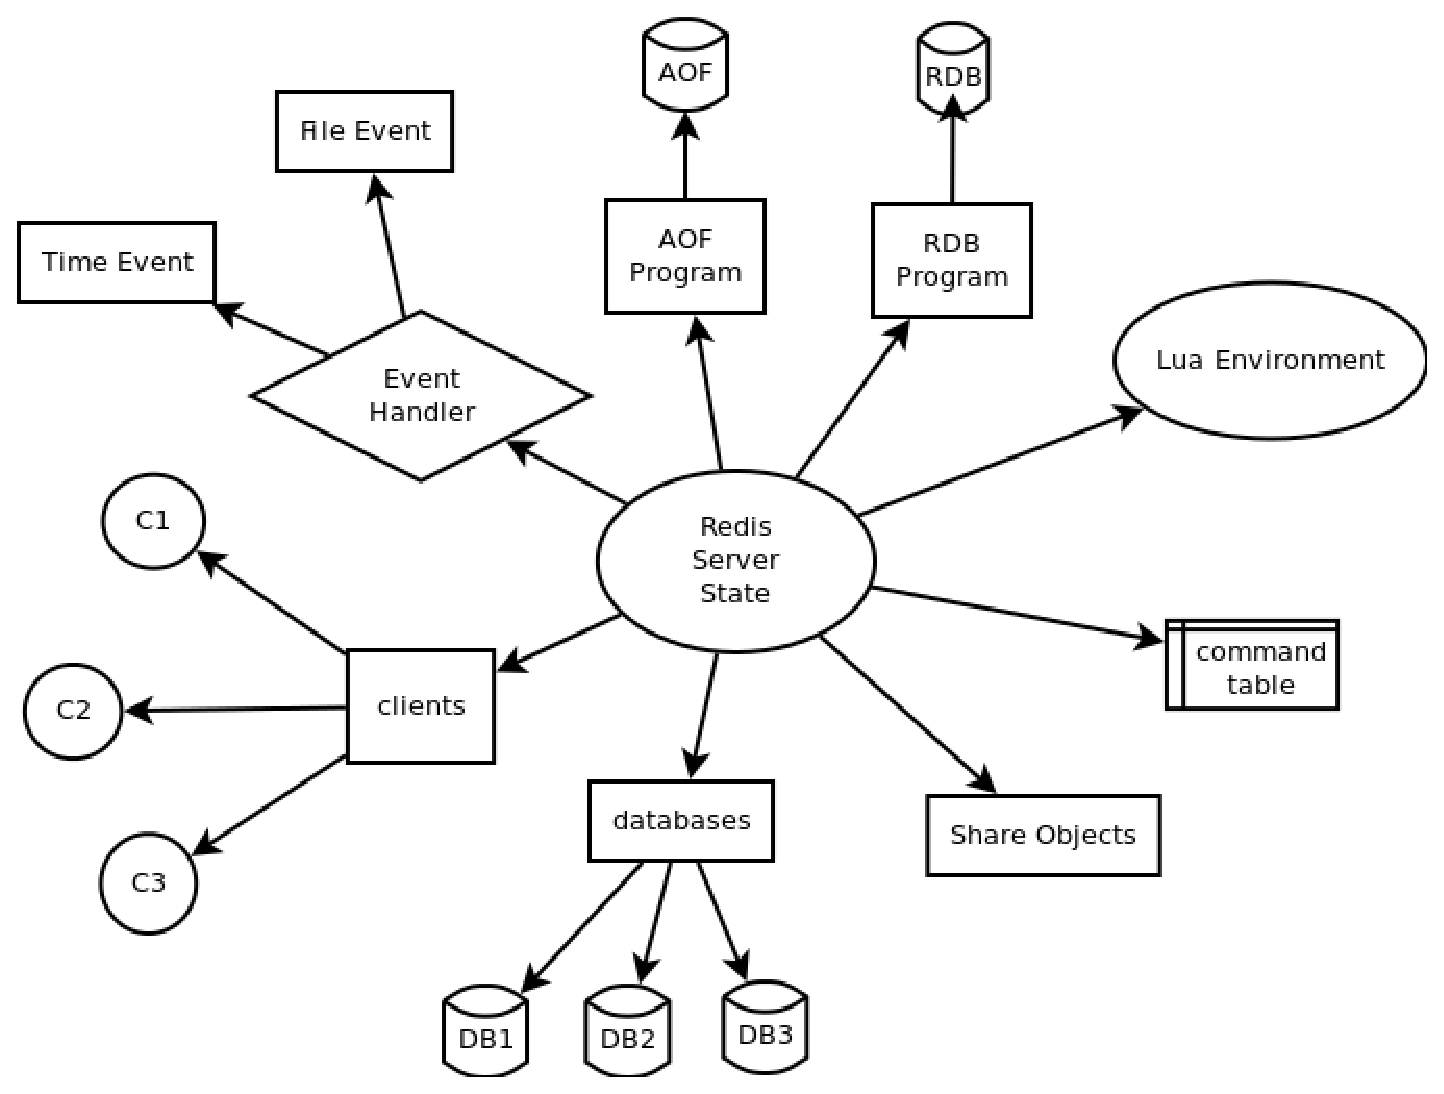
\includegraphics[width=0.4\textwidth]{redis-server}
\caption{Redis架构}\label{fig:redis-server}
\vspace{\baselineskip}
\end{figure}
}
% end Redis内部架构

\item{Redis运行流程[22]
\begin{enumerate}[label=\arabic*.]
\item{服务器初始化:从启动 Redis 服务器, 到服务器可以接受外来客户端的网络连接这段时间, Redis 需要执行一系列初始化操作。整个初始化过程可以分为六个步骤:初始化服务器全局状态→载入配置文件→创建daemon进程→初始化服务器功能模块→载入数据→开始事件循环。
}
\item{一个客户端通过Socket函数连接到服务器。}
\item{从客户端发送命令请求, 到命令被服务器处理、并将结果返回客户端。}
\end{enumerate}
}

\item{编程语言:Python\\
Python现在是最流行的动态编程语言之一,紧接着是Perl,Tcl,PHP和最近的Ruby。虽然它经常被看做是“脚本语言”,但实际上它是和List或者Smalltalk类似写法的通用编程语言。今天,python被用在很多地方,从使用完就扔的脚本到提供24x7不间断服务的大型web服务。它还用在GUI和数据库编程,客户端和服务端web编程,程序测试。
作为一种即译式的,互动的,面向对象的编程语言,它包含了模组式的操作,异常处理,动态资料形态,十分高层次的动态资料结构,以及类别的使用。Python揉合了简单的语法和强大的功能。它的语法表达优美易读。它具有很多优秀的脚本语言的特点:解释的,面向对象的,内建的高级数据结构,支持模块和包,支持多种平台,可扩展。而且它还支持交互式方式运行,图形方式运行。它拥有众多的编程界面支持各种操作系统平台以及众多的各类函数库。利用C和C++可以对它进行扩充。个别的应用软件如果需要有一个可程序化界面也可以利用它来做为扩展语言用。

}
% \begin{enumerate}[label=\Alph*.]
\end{enumerate}

\chapter{研究工作总体安排与时间进度}
\begin{table}[htbp]
\caption{工作总体安排与时间进度}\label{tab:table1}
\vspace{0.5em}
\begin{center}
{\wuhao
\begin{tabular}{|c|c|c|}
\hline
任务序号 & 起止时间 & 阶段任务要点\\ \hline
1 & 2013.1.11~-~2013.2.20 & 了解课题相关内容,查找中、英文资料\\ \hline
2 & 2013.2.21~-~2013.3.8 & 查阅文献资料,完成文献综述、开题报告和外文翻译\\ \hline
3 & 2013.3.9~-~2013.3.25 & 阅读Redis源代码,分析其架构\\ \hline
4 & 2013.3.26~-~2013.4.1 & 系统详细设计\\ \hline
5 & 2013.4.2~-~2013.4.24 & 编码\\ \hline
6 & 2013.4.25~-~2013.4.30 & 系统测试\\ \hline
7 & 2013.5.1~-~2013.5.15 & 整理资料,完成论文\\ \hline
\end{tabular}}
\end{center}
\vspace{\baselineskip}
\end{table}

\backmatter
\endgroup % 组结束
%%%%%%%%%% 参考文献 %%%%%%%%%%
\clearpage % 显式换页,使书签定位准确
\bibliography{references/reference}
\nocite{*}                                   % 若将此命令屏蔽掉,则未引用的文献不会出现在文后的参考文献中。

%%%%%%%%%% 附录 %%%%%%%%%%
%\appendix
%\include{appendix/appendix}            % 附录

\end{document}                                  % 结束全文
